% ============================================================
\chapter{Image Generation Architectures: From Convolutions to Transformers}
\label{chap:architectures}
% ============================================================

The architectural substrate of a generative model is not merely an implementation detail; it determines the inductive biases brought to bear on the data distribution, the computational complexity of training and inference, and ultimately the fidelity and diversity of the generated outputs. The rapid progress of image generation over the past decade is inseparable from a corresponding evolution in backbone architectures — from the early adoption of convolutional neural networks (CNNs) in adversarial and variational frameworks, through the emergence of U-shaped encoder-decoder networks as the workhorse of score-based and diffusion models, to the more recent integration of the self-attention mechanism and its descendant, the Vision Transformer. This chapter surveys these architectural developments with emphasis on the components most directly relevant to diffusion-based image synthesis and the knowledge distillation paradigms discussed in Chapter~\ref{chap:knowledge_distillation}.

% ============================================================
\section{Convolutional Neural Networks}
\label{sec:cnns}
% ============================================================

Convolutional neural networks, whose modern form was systematized by \cite{lecun1998gradient} and subsequently scaled to deep configurations by \cite{krizhevsky2012imagenet}, established the dominant representational paradigm for visual data throughout the 2010s. Their defining structural property is the exploitation of spatial locality and translational equivariance: a learnable filter $\mathbf{w} \in \mathbb{R}^{k \times k \times C_{\text{in}}}$ is convolved with a feature map $\mathbf{x} \in \mathbb{R}^{H \times W \times C_{\text{in}}}$ to produce an output feature map $\mathbf{y} \in \mathbb{R}^{H' \times W' \times C_{\text{out}}}$, where the same filter weights are shared across all spatial positions. Formally, the output at spatial location $(i, j)$ and output channel $c$ is

\begin{equation}
    \mathbf{y}_{i,j,c} = \sum_{c'=1}^{C_{\text{in}}} \sum_{p=0}^{k-1} \sum_{q=0}^{k-1} \mathbf{w}_{p,q,c',c} \cdot \mathbf{x}_{s \cdot i + p,\; s \cdot j + q,\; c'},
    \label{eq:convolution}
\end{equation}

where $s$ denotes the stride. This parameter-sharing scheme yields a substantially smaller model compared to a fully connected layer operating on the same input dimensions, and simultaneously encodes the prior that meaningful visual patterns can occur at arbitrary spatial locations.

Progressive downsampling via strided convolutions or pooling operations reduces the spatial resolution while increasing the number of feature channels, enabling a hierarchical extraction of features at multiple scales. Early layers respond to low-level statistics such as edges and color gradients; deeper layers encode increasingly abstract, semantically meaningful representations \cite{zeiler2014visualizing}. This multi-scale hierarchy is a property that generative architectures have deliberately preserved and exploited.

Normalization layers, principally Batch Normalization \cite{ioffe2015batch} and, later, Group Normalization \cite{wu2018group}, proved essential for stabilizing the training of deep convolutional stacks by reducing internal covariate shift. In the context of generative models conditioned on auxiliary information — such as the diffusion timestep $t$ or a class label — adaptive normalization schemes, specifically Adaptive Group Normalization and Adaptive Layer Normalization, were introduced to modulate intermediate feature representations \cite{dhariwal2021diffusion}. In these schemes, the affine parameters $(\gamma, \beta)$ of the normalization are not fixed scalars but are instead predicted from a conditioning embedding, allowing the network to adjust its internal feature statistics as a function of the condition.

% ============================================================
\subsection{U-Net and its Role in Diffusion}
\label{subsec:unet}
% ============================================================

The U-Net architecture, introduced by \cite{ronneberger2015unet} for biomedical image segmentation, represents a pivotal design pattern for tasks that require both global contextual understanding and fine-grained spatial precision. Its defining characteristic is a symmetric encoder-decoder structure augmented with skip connections that bypass the bottleneck and concatenate encoder feature maps directly to their spatially corresponding decoder feature maps.

Formally, denote the encoder as a sequence of resolution-halving blocks $\{E_\ell\}_{\ell=1}^{L}$ and the decoder as a sequence of resolution-doubling blocks $\{D_\ell\}_{\ell=1}^{L}$. The skip connection at level $\ell$ concatenates the encoder output $\mathbf{h}^{E}_\ell$ with the upsampled decoder feature $\mathbf{h}^{D}_{\ell+1}$ prior to processing by $D_\ell$:

\begin{equation}
    \mathbf{h}^{D}_{\ell} = D_\ell\!\left(\left[\mathbf{h}^{D}_{\ell+1};\; \mathbf{h}^{E}_\ell\right]\right),
    \label{eq:unet_skip}
\end{equation}

where $[\cdot\,;\,\cdot]$ denotes channel-wise concatenation. This mechanism preserves high-frequency spatial detail that would otherwise be irrecoverably lost through successive downsampling operations, enabling precise, pixel-level outputs.

The U-Net was adopted as the denoising backbone in the seminal Denoising Diffusion Probabilistic Models (DDPMs) framework of \cite{ho2020denoising}, and it has since become the near-universal architectural choice for diffusion-based image generators \cite{nichol2021improved, dhariwal2021diffusion, rombach2022latent}. Its suitability for this role stems from several complementary properties. First, the denoising task is itself a dense prediction problem: the network must predict the noise $\boldsymbol{\epsilon}$ (or, equivalently, the score $\nabla_{\mathbf{x}_t} \log p(\mathbf{x}_t)$) at every pixel of an input noisy image $\mathbf{x}_t$, which demands that spatial resolution be maintained end-to-end — precisely the function of the decoder and skip connections. Second, the multi-scale feature hierarchy naturally accommodates the multi-frequency nature of image content: low-frequency structure (overall layout, global semantics) is captured at the bottleneck, while high-frequency detail (texture, edges) is routed through the skip connections. Third, the bottleneck of the U-Net serves as a natural site for injecting conditioning information, whether temporal (the diffusion timestep $t$), semantic (a text embedding from a language model), or structural.

\begin{figure}[ht]
    \centering
    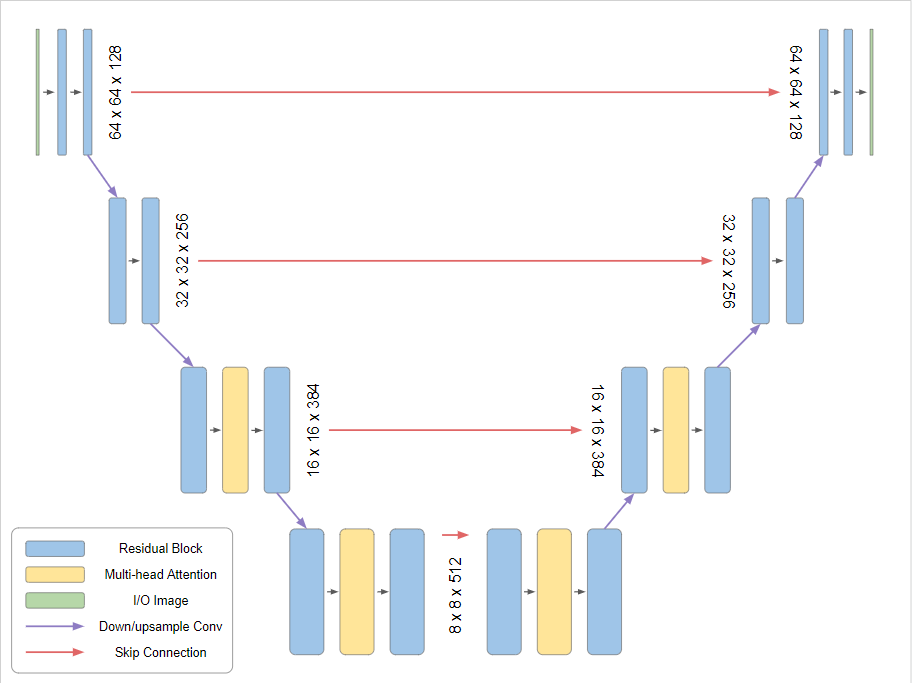
\includegraphics[width=0.85\linewidth]{figures/bcg/unetdiffusion.png}
    \caption{Schematic of a U-Net denoising backbone as employed in diffusion models. Encoder blocks (left) progressively reduce spatial resolution while expanding the channel dimension; decoder blocks (right) reverse this process. Skip connections (horizontal arrows) concatenate encoder features into the corresponding decoder stage. The timestep embedding $\tau(t)$, derived from a sinusoidal encoding, is injected via adaptive normalization at each resolution level.}
    \label{fig:unet_diffusion}
\end{figure}

The specific instantiation of the U-Net used in \cite{dhariwal2021diffusion} — which established a new state of the art for class-conditional image synthesis and whose architecture underpins much of the subsequent work on distillation — departs from the original segmentation-oriented design in several important respects. Each resolution level consists of multiple residual blocks \cite{he2016deep} rather than single convolutional layers, providing increased representational capacity at each scale without altering the spatial resolution. Self-attention layers (discussed in Section~\ref{sec:attention}) are interleaved with the convolutional residual blocks, initially only at the lowest-resolution levels where the global receptive field of attention is computationally tractable, but extending to higher resolutions in the largest model variants. Timestep conditioning is implemented by computing a sinusoidal positional embedding of $t$, projecting it through a small feed-forward network, and using the result to modulate the affine parameters of Group Normalization layers via Adaptive Group Normalization. This architecture served as the direct predecessor to the latent diffusion model U-Nets \cite{rombach2022latent}, and variants of it are employed in many of the knowledge distillation frameworks surveyed in Chapter~\ref{chap:knowledge_distillation}.

% ============================================================
\section{The Attention Mechanism}
\label{sec:attention}
% ============================================================

The attention mechanism, first introduced in the context of sequence-to-sequence neural machine translation by \cite{bahdanau2015neural} and subsequently generalized into the Transformer architecture by \cite{vaswani2017attention}, represents a fundamentally different computational primitive from convolution. Whereas a convolutional filter aggregates information within a fixed local neighborhood, an attention layer computes a weighted aggregation over all positions in a feature map, with the weights themselves being input-dependent. This endows attention-based models with a global receptive field at every layer and the capacity to model long-range dependencies that require many stacked convolutional layers to capture, if they are captured at all.

% ============================================================
\subsection{Self-Attention}
\label{subsec:self_attention}
% ============================================================

In the self-attention formulation, a single input sequence $\mathbf{X} \in \mathbb{R}^{N \times d}$, consisting of $N$ tokens each of dimension $d$, is linearly projected into three distinct representations: the query matrix $\mathbf{Q} = \mathbf{X}\mathbf{W}^Q$, the key matrix $\mathbf{K} = \mathbf{X}\mathbf{W}^K$, and the value matrix $\mathbf{V} = \mathbf{X}\mathbf{W}^V$, where $\mathbf{W}^Q, \mathbf{W}^K, \mathbf{W}^V \in \mathbb{R}^{d \times d_k}$ are learned projection matrices. The attention output is then computed as

\begin{equation}
    \text{Attention}(\mathbf{Q}, \mathbf{K}, \mathbf{V}) = \text{softmax}\!\left(\frac{\mathbf{Q}\mathbf{K}^\top}{\sqrt{d_k}}\right)\mathbf{V},
    \label{eq:self_attention}
\end{equation}

where the factor $\sqrt{d_k}$ is a scaling constant introduced to prevent the dot products from growing too large in magnitude and saturating the softmax function \cite{vaswani2017attention}. The $(i, j)$-th entry of the pre-softmax matrix $\mathbf{Q}\mathbf{K}^\top / \sqrt{d_k}$ can be interpreted as an unnormalized compatibility score between position $i$ and position $j$. After row-wise softmax normalization, these scores form a probability distribution over positions, and the output at position $i$ is a convex combination of all value vectors, weighted by the compatibility of position $i$ with every other position. The computational complexity of this operation is $\mathcal{O}(N^2 d_k)$, which is the primary practical limitation of self-attention when applied to high-resolution images.

When self-attention is applied to two-dimensional feature maps $\mathbf{F} \in \mathbb{R}^{H \times W \times C}$, the spatial dimensions are first flattened into a sequence of $N = H \times W$ tokens, each of dimension $C$. The attention computation then proceeds as described above, after which the output is reshaped back to $\mathbb{R}^{H \times W \times C}$. The quadratic cost in $N$ explains why, in the U-Nets used for diffusion, full self-attention is typically applied only at the lowest-resolution feature maps (e.g., $8 \times 8$ or $16 \times 16$), where $N$ is small, while higher-resolution stages rely on convolutional blocks. Efficient variants such as linear attention \cite{katharopoulos2020transformers} and window-based local attention \cite{liu2021swin} have been proposed to mitigate this bottleneck, and several of these are employed in more recent diffusion architectures.

% ============================================================
\subsection{Multi-Head and Cross-Attention}
\label{subsec:multihead_cross_attention}
% ============================================================

A single attention head, as defined in Equation~\ref{eq:self_attention}, is constrained to learn a single query-key compatibility function operating in a $d_k$-dimensional subspace. Multi-head attention \cite{vaswani2017attention} overcomes this limitation by executing $H$ independent attention computations in parallel, each in a lower-dimensional subspace of dimension $d_k = d / H$, and concatenating their outputs before a final linear projection:

\begin{equation}
    \text{MultiHead}(\mathbf{Q}, \mathbf{K}, \mathbf{V}) = \left[\text{head}_1; \cdots; \text{head}_H\right]\mathbf{W}^O,
    \label{eq:multihead}
\end{equation}

where $\text{head}_h = \text{Attention}(\mathbf{X}\mathbf{W}^Q_h, \mathbf{X}\mathbf{W}^K_h, \mathbf{X}\mathbf{W}^V_h)$ and $\mathbf{W}^O \in \mathbb{R}^{d \times d}$ is the output projection. Empirically, different attention heads specialize in capturing different relational patterns — some may attend to syntactically proximate tokens, others to semantically related but spatially distant regions — and their combination yields richer representations than any single head \cite{voita2019analyzing}.

Cross-attention generalizes the self-attention mechanism to settings in which the queries are derived from one sequence and the keys and values from a distinct, conditioning sequence. Given a primary feature map $\mathbf{Z} \in \mathbb{R}^{N \times d}$ and a conditioning context $\mathbf{C} \in \mathbb{R}^{M \times d_c}$, the cross-attention output is

\begin{equation}
    \text{CrossAttention}(\mathbf{Z}, \mathbf{C}) = \text{softmax}\!\left(\frac{(\mathbf{Z}\mathbf{W}^Q)(\mathbf{C}\mathbf{W}^K)^\top}{\sqrt{d_k}}\right)(\mathbf{C}\mathbf{W}^V),
    \label{eq:cross_attention}
\end{equation}

where $\mathbf{W}^Q \in \mathbb{R}^{d \times d_k}$, $\mathbf{W}^K, \mathbf{W}^V \in \mathbb{R}^{d_c \times d_k}$. In this formulation, each position in the primary sequence $\mathbf{Z}$ attends over all $M$ positions in the conditioning sequence $\mathbf{C}$, effectively allowing information to flow from the condition into the primary representation. This mechanism is the architectural foundation of text-conditioned image generation: in Latent Diffusion Models \cite{rombach2022latent} and their successors, the text prompt is encoded by a pre-trained language model (e.g., CLIP \cite{radford2021learning} or T5 \cite{raffel2020exploring}) into a sequence of token embeddings $\mathbf{C}$, and cross-attention layers within the U-Net denoising backbone enable the model to align generated visual features with textual semantics at every resolution stage. The interaction between the visual and linguistic modalities through cross-attention has proven to be a highly expressive conditioning mechanism, and its parameters are among the primary targets of investigation in text-to-image distillation methods \cite{meng2023distillation}.

\begin{figure}[ht]
    \centering
    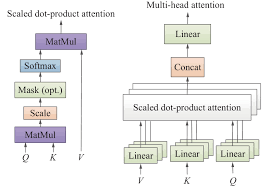
\includegraphics[width=0.80\linewidth]{figures/bcg/attention.png}
    \caption{Illustration of (a) scaled dot-product self-attention, (b) multi-head self-attention, and (c) cross-attention. In cross-attention, queries $\mathbf{Q}$ are projected from the visual feature sequence while keys $\mathbf{K}$ and values $\mathbf{V}$ are projected from the conditioning text embedding sequence $\mathbf{C}$, enabling each spatial position to selectively aggregate information from the text tokens.}
    \label{fig:attention_mechanisms}
\end{figure}

\section{The Transformer Architecture}
\label{sec:transformer}

The Transformer architecture, introduced by Vaswani et al.\ \cite{vaswani2017attention}, constitutes a paradigm shift in the design of deep neural networks for sequence modelling. Prior to its introduction, the dominant approaches for processing sequential data relied on recurrent neural networks (RNNs) and their gated variants, such as Long Short-Term Memory networks (LSTMs) \cite{hochreiter1997long} and Gated Recurrent Units (GRUs) \cite{cho2014learning}. These architectures suffer from an inherent sequential computation bottleneck: hidden states must be propagated step-by-step along the temporal axis, which prevents efficient parallelisation and impedes the capture of long-range dependencies due to vanishing gradient phenomena. The Transformer addresses both limitations by dispensing with recurrence entirely and replacing it with a mechanism of \emph{scaled dot-product attention}, enabling each position in a sequence to attend directly to every other position in a single computational step.

Formally, the core operation of the Transformer is the \emph{multi-head self-attention} mechanism. Given an input sequence represented as a matrix $\mathbf{X} \in \mathbb{R}^{n \times d_{\text{model}}}$, where $n$ is the sequence length and $d_{\text{model}}$ is the model dimensionality, three distinct linear projections produce the query, key, and value matrices:
\begin{equation}
    \mathbf{Q} = \mathbf{X}\mathbf{W}^Q, \quad
    \mathbf{K} = \mathbf{X}\mathbf{W}^K, \quad
    \mathbf{V} = \mathbf{X}\mathbf{W}^V,
    \label{eq:qkv}
\end{equation}
where $\mathbf{W}^Q, \mathbf{W}^K \in \mathbb{R}^{d_{\text{model}} \times d_k}$ and $\mathbf{W}^V \in \mathbb{R}^{d_{\text{model}} \times d_v}$ are learnable weight matrices. The attention output is then computed as:
\begin{equation}
    \text{Attention}(\mathbf{Q}, \mathbf{K}, \mathbf{V}) = \text{softmax}\!\left(\frac{\mathbf{Q}\mathbf{K}^\top}{\sqrt{d_k}}\right)\mathbf{V},
    \label{eq:attention}
\end{equation}
where the scaling factor $\sqrt{d_k}$ prevents the inner products from growing excessively large in magnitude, which would saturate the softmax function into near-zero gradient regions. In practice, multi-head attention runs $h$ parallel attention heads, each operating in a lower-dimensional subspace of dimension $d_k = d_v = d_{\text{model}} / h$, and their outputs are concatenated and linearly projected back to $d_{\text{model}}$:
\begin{equation}
    \text{MultiHead}(\mathbf{Q}, \mathbf{K}, \mathbf{V}) =
    \text{Concat}(\text{head}_1, \ldots, \text{head}_h)\,\mathbf{W}^O,
    \label{eq:multihead}
\end{equation}
where $\text{head}_i = \text{Attention}(\mathbf{X}\mathbf{W}_i^Q, \mathbf{X}\mathbf{W}_i^K, \mathbf{X}\mathbf{W}_i^V)$ and $\mathbf{W}^O \in \mathbb{R}^{h d_v \times d_{\text{model}}}$. This multi-head formulation allows the model to jointly attend to information from different representation subspaces at different positions, enriching the learned representations.

Each Transformer layer consists of two sub-layers: (i) the multi-head self-attention mechanism defined above and (ii) a position-wise feed-forward network (FFN) applied independently to each sequence position:
\begin{equation}
    \text{FFN}(\mathbf{z}) = \max(0, \mathbf{z}\mathbf{W}_1 + \mathbf{b}_1)\mathbf{W}_2 + \mathbf{b}_2,
    \label{eq:ffn}
\end{equation}
where $\mathbf{W}_1 \in \mathbb{R}^{d_{\text{model}} \times d_{\text{ff}}}$, $\mathbf{W}_2 \in \mathbb{R}^{d_{\text{ff}} \times d_{\text{model}}}$, and $d_{\text{ff}}$ is typically set to $4 d_{\text{model}}$. Residual connections \cite{he2016deep} wrap each sub-layer, followed by Layer Normalisation \cite{ba2016layer}, producing the standard pre-norm or post-norm Transformer block. Because the attention mechanism is inherently permutation-equivariant and thus insensitive to the order of input elements, positional information must be explicitly injected. The original formulation uses fixed sinusoidal encodings, though learned positional embeddings and more sophisticated relative positional schemes have been subsequently proposed \cite{shaw2018self, su2024roformer}.

The self-attention computation has a time and memory complexity of $\mathcal{O}(n^2 d_{\text{model}})$ with respect to sequence length $n$, which poses scalability challenges for long sequences. This quadratic bottleneck has motivated a rich body of work on efficient attention variants, including sparse attention \cite{child2019generating}, linear attention approximations \cite{katharopoulos2020transformers}, and hierarchical attention schemes. Notwithstanding this limitation, the Transformer has become the \emph{de facto} backbone for a broad range of tasks spanning natural language processing, speech, and, increasingly, computer vision and generative modelling, owing to its strong inductive biases towards long-range dependency modelling and its excellent scalability with respect to model size and training data.

% ============================================================
%  Section: Vision Transformers (ViT)
% ============================================================

\section{Vision Transformers}
\label{sec:vit}

The extension of the Transformer architecture to the visual domain was systematically explored by Dosovitskiy et al.\ \cite{dosovitskiy2020image}, who demonstrated that a pure Transformer applied directly to sequences of image patches can achieve competitive or superior performance compared to convolutional neural networks (CNNs) on image recognition benchmarks, provided that sufficient training data are available. This model, known as the Vision Transformer (ViT), challenged the long-standing dominance of convolutional architectures in computer vision and stimulated a proliferation of Transformer-based methods across discriminative and generative visual tasks alike.

\begin{figure}[ht]
    \centering
    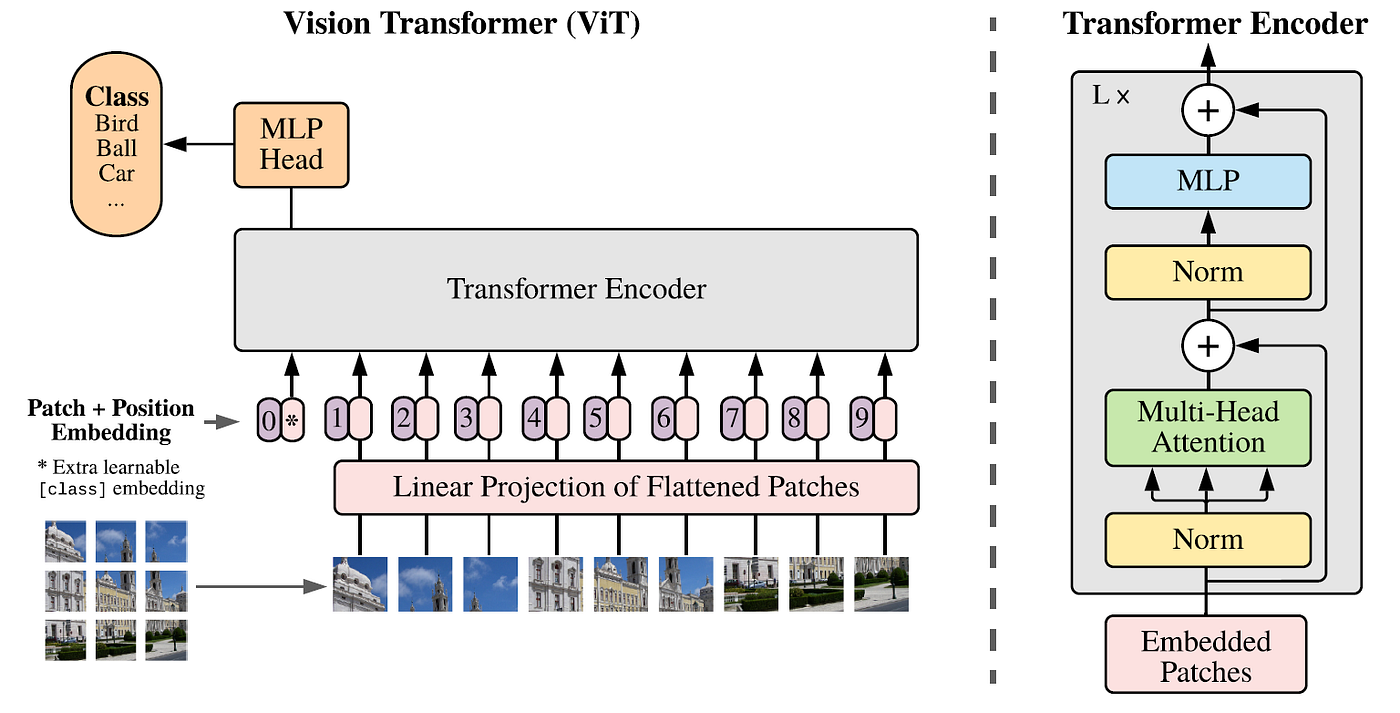
\includegraphics[width=0.85\linewidth]{figures/bcg/VIT.png}
    \caption{Overview of the Vision Transformer (ViT) architecture. An input image is partitioned into a grid of fixed-size patches, each linearly projected into a patch embedding. A learnable \texttt{[CLS]} token is prepended, positional embeddings are added, and the resulting sequence is processed by a stack of standard Transformer encoder blocks. The representation at the \texttt{[CLS]} token is used for classification. Figure adapted from \cite{dosovitskiy2020image}.}
    \label{fig:vit_architecture}
\end{figure}

% ============================================================
%  Subsection: Patch Embeddings and Positional Encoding
% ============================================================

\subsection{Patch Embeddings and Positional Encoding}
\label{subsec:patch_embeddings}

The principal challenge in applying Transformers to images lies in managing the computational cost of the quadratic attention mechanism. A raw image $\mathbf{x} \in \mathbb{R}^{H \times W \times C}$, if naively unrolled into a sequence of individual pixels, would yield a sequence of length $n = HW$, rendering self-attention computationally intractable for any practical image resolution. ViT resolves this by partitioning the image into a grid of non-overlapping patches of fixed size $P \times P$, resulting in $n = HW / P^2$ patches. Each patch $\mathbf{x}_i \in \mathbb{R}^{P^2 C}$ is then linearly projected into a $d_{\text{model}}$-dimensional embedding space via a learnable matrix $\mathbf{E} \in \mathbb{R}^{P^2 C \times d_{\text{model}}}$:
\begin{equation}
    \mathbf{z}_i^{(0)} = \mathbf{x}_i \mathbf{E} + \mathbf{e}_i^{\text{pos}},
    \quad i = 1, \ldots, n,
    \label{eq:patch_embedding}
\end{equation}
where $\mathbf{e}_i^{\text{pos}} \in \mathbb{R}^{d_{\text{model}}}$ is the positional embedding associated with the $i$-th position. Equivalently, the linear projection $\mathbf{E}$ can be implemented as a strided $P \times P$ convolution with $d_{\text{model}}$ output channels and stride $P$, which establishes a conceptual bridge to convolutional feature extraction.

A learnable classification token $\mathbf{z}_{\text{cls}} \in \mathbb{R}^{d_{\text{model}}}$, prepended to the patch sequence following the BERT convention \cite{devlin2019bert}, aggregates global image information through the attention mechanism. The full input sequence to the Transformer encoder is thus:
\begin{equation}
    \mathbf{Z}^{(0)} = \left[\mathbf{z}_{\text{cls}};\, \mathbf{z}_1^{(0)};\, \ldots;\, \mathbf{z}_n^{(0)}\right] \in \mathbb{R}^{(n+1) \times d_{\text{model}}}.
    \label{eq:vit_input}
\end{equation}
This sequence is then processed by $L$ stacked Transformer encoder blocks, each applying multi-head self-attention as described in Section~\ref{sec:transformer}, followed by a layer-normalised FFN with residual connections.

Positional encoding in ViT is typically realised through \emph{learned} 1D positional embeddings $\{\mathbf{e}_i^{\text{pos}}\}_{i=0}^{n}$, one for each patch position (plus the class token). Empirical comparisons reported in \cite{dosovitskiy2020image} indicate that 1D learned embeddings perform comparably to 2D-aware positional schemes for standard image resolutions, suggesting that the Transformer is capable of inferring 2D spatial relationships from 1D position information given sufficient data. More recent work has proposed relative positional encodings \cite{shaw2018self} and rotary positional embeddings (RoPE) \cite{su2024roformer} for ViT-style models, particularly to improve generalisation to image resolutions not seen during training — a practically important property for generative applications where spatial resolution may vary.

% ============================================================
%  Subsection: Scalability and Inductive Bias
% ============================================================

\subsection{Scalability and Inductive Bias}
\label{subsec:vit_scalability}

A defining characteristic of ViT relative to CNN-based architectures is its substantially weaker set of built-in inductive biases. Convolutional networks impose locality (each filter operates on a spatially contiguous receptive field), translation equivariance (a feature detector applied at one spatial location is reused across the entire feature map), and weight sharing. These structural priors are highly effective for natural image data and enable CNNs to generalise well even in data-limited regimes. The Transformer, in contrast, makes no structural assumptions about the spatial arrangement of its input tokens: every pair of patch tokens can interact with every other pair through the global attention mechanism, irrespective of their spatial distance. This architectural agnosticism is a double-edged property: it renders the model highly expressive and capable of capturing global dependencies that local convolutions cannot model efficiently, but it also necessitates substantially larger training datasets to learn the relevant spatial regularities that convolutional architectures acquire as an architectural prior.

This interplay between inductive bias and data scale is reflected empirically in the scaling behaviour of ViT. When trained on moderately sized datasets such as ImageNet-1k (${\sim}1.2$ million images), ViT lags behind well-regularised CNNs such as ResNet and EfficientNet \cite{he2016deep, tan2019efficientnet} in classification accuracy. However, when pre-trained on substantially larger corpora — in the order of hundreds of millions or billions of images — ViT models consistently outperform CNN counterparts \cite{dosovitskiy2020image, zhai2022scaling}. This observation motivates a shift in the design philosophy for large-scale vision models: rather than engineering architectural priors, one invests in data and compute, relying on the expressivity of the attention mechanism to discover the relevant structure from data.

The scalability of ViT is further underscored by the near-linear relationship between model capacity and downstream performance observed across multiple orders of magnitude in parameter count, from ViT-Small (${\sim}22$M parameters) through ViT-Base (${\sim}86$M) and ViT-Large (${\sim}307$M) to ViT-Huge (${\sim}632$M) and beyond \cite{zhai2022scaling}. This predictable scaling behaviour stands in contrast to CNN architectures, for which performance improvements tend to saturate more rapidly with increasing depth or width. Consequently, ViT has become the preferred backbone for foundation model pre-training in vision, underpinning models such as DINO \cite{caron2021emerging}, MAE \cite{he2022masked}, and CLIP \cite{radford2021learning}, all of which are directly relevant to the construction of powerful visual representations for downstream generative tasks.

% ============================================================
%  Subsection: Adapting ViT to Generative Tasks
% ============================================================

\subsection{Adapting ViT to Generative Tasks}
\label{subsec:vit_generative}

The success of ViT as a discriminative backbone has prompted extensive investigation into its utility as a backbone for generative modelling. This adaptation is non-trivial, as generative models impose architectural requirements that differ substantially from classification: they must produce spatially coherent, high-resolution outputs, and they must condition their generation on auxiliary signals such as class labels, text embeddings, or noisy latent states. Several strategies have emerged for repurposing the ViT architecture in this setting.

The most direct adaptation employs ViT as the denoising network within a diffusion model framework. The Diffusion Transformer (DiT), proposed by Peebles and Xie \cite{peebles2023scalable}, replaces the U-Net backbone conventionally used in denoising diffusion probabilistic models \cite{ho2020denoising} with a pure Transformer operating on sequences of latent image patches. DiT operates in the latent space of a pre-trained variational autoencoder (VAE), accepting as input the noisy latent $\mathbf{z}_t \in \mathbb{R}^{h \times w \times c}$ at diffusion timestep $t$, which is tokenised into a sequence of $n = hw/P^2$ patch tokens. Conditioning on the diffusion timestep $t$ and an optional class label $y$ is achieved through \emph{adaptive layer normalisation} (adaLN), wherein the scale and shift parameters of each layer normalisation are predicted by a small MLP applied to the sum of the timestep embedding and the class embedding:
\begin{equation}
    \text{adaLN}(\mathbf{h}, t, y) = \boldsymbol{\gamma}(t, y) \odot \frac{\mathbf{h} - \mu(\mathbf{h})}{\sigma(\mathbf{h})} + \boldsymbol{\beta}(t, y),
    \label{eq:adaln}
\end{equation}
where $\boldsymbol{\gamma}(t, y), \boldsymbol{\beta}(t, y) \in \mathbb{R}^{d_{\text{model}}}$ are the predicted scale and shift vectors, $\odot$ denotes element-wise multiplication, and $\mu$, $\sigma$ denote the mean and standard deviation computed over the feature dimension. This conditioning mechanism is more expressive than simple token concatenation and has been shown to be critical for the quality of conditional image synthesis.

\begin{figure}[ht]
    \centering
    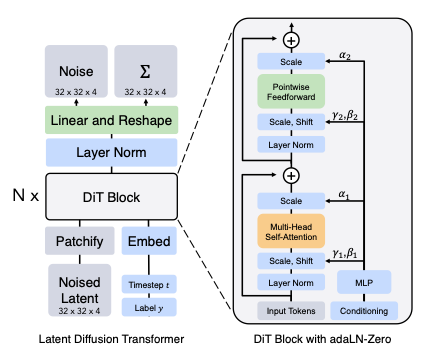
\includegraphics[width=0.85\linewidth]{figures/bcg/DIT-ADA.png}
    \caption{Schematic of a DiT block with adaptive layer normalization (adaLN). Conditioning signals from the diffusion timestep embedding and optional class label are used to modulate the layer normalization parameters $\boldsymbol{\gamma}$ and $\boldsymbol{\beta}$, providing flexible conditional control over the denoising process \cite{peebles2023scalable}.}
    \label{fig:dit_block}
\end{figure}

DiT exhibits the same favourable scaling properties as discriminative ViT: larger models trained for longer consistently achieve lower FID scores on class-conditional ImageNet generation, with DiT-XL/2 (trained at $256 \times 256$ resolution) surpassing all prior diffusion models including those based on U-Net backbones \cite{peebles2023scalable}. This scalability is particularly germane to the subject of the present thesis, as the Transformer backbone makes DiT an attractive target for knowledge distillation: the clean, modular structure of Transformer layers facilitates the design of intermediate feature-matching objectives, and the availability of a family of models at different scales (DiT-S, DiT-B, DiT-L, DiT-XL) provides natural student-teacher pairs that share an identical architectural template, differing only in depth and width.

Beyond DiT, other generative Transformer variants have been proposed. The U-ViT architecture \cite{bao2023all} hybridises the U-Net skip-connection topology with a Transformer backbone, introducing long skip connections between shallow and deep Transformer blocks to facilitate multi-scale feature propagation — a design motivated by the observation that low-frequency spatial information is most effectively communicated through direct shortcuts rather than through the deep processing stack. More recently, Flux and related flow-matching models \cite{lipman2022flow, esser2024scaling} have adopted Transformer-based backbones with multi-modal attention streams, enabling joint processing of image and text tokens within a unified attention computation. These architectures represent the current state of the art in text-to-image synthesis and are directly relevant to the distillation methodologies examined in Chapter~\ref{chap:knowledge_distillation}.

% ================================================================
% SECTION: The Just Image Transformer (JiT)
% ================================================================

\section{The Just Image Transformer (JiT)}
\label{sec:jit}

The Just image Transformer (JiT), introduced by \cite{li2025jit}, represents a principled return to the foundational objective of denoising generative models: directly predicting clean data rather than noise or a noised quantity. Despite the apparent simplicity of this design choice, it carries profound consequences for how neural networks handle high-dimensional image spaces. The JiT framework demonstrates that a plain Vision Transformer (ViT) operating directly on raw pixel patches — without any latent tokenizer, adversarial loss, perceptual loss, or self-supervised pre-training — can serve as a powerful and competitive generative backbone, provided the network is tasked with predicting the clean image $\bm{x}$ rather than the noise $\bm{\epsilon}$ or the flow velocity $\bm{v}$. This section details the theoretical motivation underpinning this design philosophy, the architectural choices that realise it, and the diffusion and flow-matching formulation within which JiT operates.

% ----------------------------------------------------------------
\subsection{The Manifold Assumption and the x-Prediction}
\label{subsec:jit_manifold}

A central premise of the JiT framework is the \emph{manifold hypothesis}, a long-standing conjecture in machine learning and statistics asserting that high-dimensional observational data, such as natural images, reside approximately on a low-dimensional nonlinear manifold embedded within the ambient observation space \cite{chapelle2006semi, carlsson2009topology, roweis2000nonlinear, tenenbaum2000global}. Formally, if $\bm{x} \in \mathbb{R}^D$ denotes a natural image of dimensionality $D$ (e.g., $D = 256 \times 256 \times 3 = 196{,}608$ for a colour image), the manifold hypothesis posits the existence of an intrinsic dimension $d \ll D$ such that the data distribution $p_{\mathrm{data}}(\bm{x})$ is supported on a $d$-dimensional submanifold $\mathcal{M} \subset \mathbb{R}^D$.

The implications of this hypothesis for diffusion model training are stark and have been largely overlooked in prior literature. In a standard Gaussian diffusion process, the noised intermediate variable at time $t$ is:
\begin{equation}
    \bm{z}_t = a_t \bm{x} + b_t \bm{\epsilon},
    \label{eq:jit_noisy}
\end{equation}
where $\bm{\epsilon} \sim \mathcal{N}(\bm{0}, \bm{I})$ is pure Gaussian noise and $a_t, b_t \in \mathbb{R}$ are pre-defined noise schedule coefficients. While the clean image $\bm{x}$ lies approximately on $\mathcal{M}$, both the noise $\bm{\epsilon}$ and the flow velocity $\bm{v} = \bm{x} - \bm{\epsilon}$ are inherently distributed across the full ambient space $\mathbb{R}^D$, as they involve an isotropic Gaussian component that fills the entire high-dimensional space \cite{vincent2010stacked}. This distinction is illustrated schematically in Figure~\ref{fig:jit_manifold}.

\begin{figure}[ht]
    \centering
    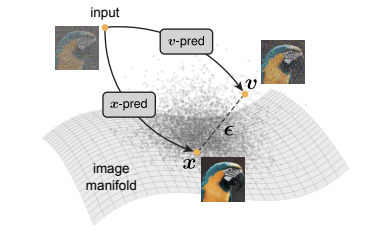
\includegraphics[width=0.72\linewidth]{figures/bcg/Manifold.png}
    \caption{c. A clean image $\bm{x}$ resides approximately on the low-dimensional data manifold $\mathcal{M}$ embedded within the high-dimensional pixel space $\mathbb{R}^D$. In contrast, the noise $\bm{\epsilon}$ and flow velocity $\bm{v} = \bm{x} - \bm{\epsilon}$ are off-manifold, distributed throughout $\mathbb{R}^D$. Training a network to predict $\bm{x}$ ($\bm{x}$-prediction) is therefore fundamentally different from training it to predict $\bm{\epsilon}$ or $\bm{v}$ (adapted from \cite{li2025jit}).}
    \label{fig:jit_manifold}
\end{figure}

This geometric insight has a direct consequence for neural network capacity. A network that must predict $\bm{\epsilon}$ is compelled to faithfully represent a full-dimensional Gaussian vector; it must retain all $D$ degrees of freedom of the noise, since any loss of information corrupts the prediction. In contrast, a network predicting $\bm{x}$ need only capture the $d$-dimensional structure of the data manifold and suppress the off-manifold noise components. Remarkably, this implies that even an \emph{under-capacity} network — one whose hidden dimension is smaller than the ambient dimension $D$ — can still perform $\bm{x}$-prediction effectively, because the information it must preserve is intrinsically low-dimensional.

\cite{li2025jit} verify this claim through a controlled toy experiment. A $d$-dimensional latent variable $\hat{\bm{x}} \in \mathbb{R}^d$ is embedded into an observed space of dimension $D \gg d$ via a fixed, randomly drawn column-orthogonal projection matrix $P \in \mathbb{R}^{D \times d}$, yielding $\bm{x} = P\hat{\bm{x}}$. A five-layer ReLU multilayer perceptron (MLP) with 256 hidden units is then trained as a generative model under $\bm{x}$-, $\bm{\epsilon}$-, and $\bm{v}$-prediction, all using the flow velocity loss (detailed in Section~\ref{subsec:jit_diffusion}). For small $D$ (e.g., $D = 2$ or $D = 8$), all three prediction modes perform reasonably. However, as $D$ increases to 16 and catastrophically to $D = 512$, $\bm{\epsilon}$-prediction and $\bm{v}$-prediction degrade severely, while $\bm{x}$-prediction continues to succeed — even though the MLP is strictly under-complete relative to the ambient space. This empirical finding is consistent with the manifold-theoretic argument: only $\bm{x}$-prediction respects the intrinsic dimensionality of the data, freeing the network from having to model the full high-dimensional noise distribution.

The broader context for this distinction can be traced to the prior literature on denoising autoencoders (DAEs) \cite{vincent2008extracting, vincent2010stacked}, where directly predicting clean data from corrupted observations was explicitly motivated by the manifold assumption. However, when \cite{ho2020denoising} demonstrated that $\bm{\epsilon}$-prediction dramatically outperformed $\bm{x}$-prediction within the DDPM framework, the field largely abandoned direct clean-image prediction. \cite{li2025jit} argue that this historical choice was appropriate in lower-dimensional regimes (e.g., latent spaces of dimensionality $\sim 64$–$256$ per token) where the capacity constraint is not binding, but becomes critically detrimental in the high-dimensional pixel space, where per-patch dimensionalities can reach 768 or 3072 depending on the patch size.

Furthermore, popular remedies for the high-dimensionality problem — such as reweighting the training loss, shifting the noise schedule, or increasing the network width — are shown by \cite{li2025jit} to be insufficient. Reweighting adjusts which noise levels receive more gradient signal but does not alter the fundamental capacity requirement for noise prediction. Increasing the network width proportionally to the token dimension rapidly becomes computationally intractable as resolution and patch size grow. The only principled remedy, JiT argues, is to change the prediction target itself.

% ----------------------------------------------------------------
\subsection{Architecture Overview: A Self-Contained ViT}
\label{subsec:jit_architecture}

The architectural design of JiT deliberately eschews the layers of specialisation that have accumulated in modern diffusion pipelines. Contemporary state-of-the-art image generators typically rely on a cascade of components: a pre-trained variational autoencoder (VAE) or vector-quantised tokeniser to project images into a compact latent space \cite{rombach2022ldm}, followed by adversarial or perceptual auxiliary losses drawn from pre-trained discriminators or classifiers \cite{goodfellow2014generative, zhang2018unreasonable}, and increasingly on self-supervised representation alignment objectives \cite{chen2024repa}. JiT eliminates all of these, operating entirely in raw pixel space with a single training objective and no external supervisory signal.

Formally, let $\bm{x} \in \mathbb{R}^{H \times W \times C}$ denote an input image of spatial dimensions $H \times W$ and $C = 3$ colour channels. JiT divides the image into non-overlapping square patches of side length $p$, yielding a sequence of $N = \frac{H}{p} \times \frac{W}{p}$ tokens, each of dimension $p^2 C$. For the canonical JiT/16 and JiT/32 configurations benchmarked on ImageNet at $256 \times 256$ and $512 \times 512$ resolutions respectively, the per-token dimensionalities are:
\begin{equation}
    d_{\text{token}} = p^2 C = \begin{cases} 16^2 \times 3 = 768 & \text{(JiT/16 at } 256 \times 256\text{)}, \\ 32^2 \times 3 = 3072 & \text{(JiT/32 at } 512 \times 512\text{)}. \end{cases}
    \label{eq:jit_token_dim}
\end{equation}
These dimensionalities are comparable to or substantially larger than those encountered in standard latent diffusion pipelines, where per-token latent dimensionalities are typically 4–16 \cite{rombach2022ldm, esser2024sd3}.

Each token is linearly projected into the Transformer's hidden dimension $d_{\text{model}}$ via a learned embedding matrix $W_e \in \mathbb{R}^{p^2 C \times d_{\text{model}}}$. Absolute sinusoidal positional embeddings are added, following the original ViT formulation \cite{dosovitskiy2021vit}. The sequence is then processed by $L$ standard Transformer blocks, each consisting of multi-head self-attention (MHSA) and a position-wise feed-forward network (FFN), with pre-normalisation via layer norm \cite{ba2016layer}. An output linear predictor $W_o \in \mathbb{R}^{d_{\text{model}} \times p^2 C}$ maps each output token back to a $p^2 C$-dimensional patch prediction. The complete pipeline is summarised in Figure~\ref{fig:jit_architecture}.

\begin{figure}[ht]
    \centering
    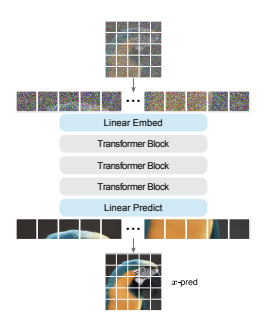
\includegraphics[width=0.78\linewidth]{figures/bcg/JIT.png}
    \caption{The JiT architecture. A noisy image $\bm{z}_t$ is patchified into a sequence of $N$ tokens, linearly embedded, processed by $L$ standard Transformer blocks conditioned on the diffusion time $t$ and class label $c$ via adaLN-Zero, and decoded back to pixel patches via a linear predictor. The direct output of the network is the clean image prediction $\hat{\bm{x}}_\theta$.}
    \label{fig:jit_architecture}
\end{figure}

Conditioning on the diffusion time step $t \in [0, 1]$ and, for class-conditional generation, on a class embedding $c$, is achieved through the adaptive layer normalisation with zero initialisation (adaLN-Zero) mechanism, as introduced by \cite{peebles2023dit}. In this formulation, time and class embeddings are combined and used to predict per-channel scale and shift parameters for the layer normalisation operations within each Transformer block, as well as a gating scalar applied to the residual branch outputs. The gate is initialised to zero, ensuring that the Transformer begins training as an identity mapping. Formally, for a hidden representation $\bm{h}$ at a given block:
\begin{equation}
    \bm{h} \leftarrow \bm{h} + \gamma \cdot \mathrm{Block}\!\left(\alpha \cdot \frac{\bm{h} - \mu}{\sigma} + \beta\right),
    \label{eq:adaln}
\end{equation}
where $\mu, \sigma$ are the layer-wise mean and standard deviation, and $\alpha, \beta, \gamma \in \mathbb{R}^{d_{\text{model}}}$ are affine parameters predicted from the joint time-class conditioning vector.

A notable finding from \cite{li2025jit} concerns the relationship between the network's hidden dimension $d_{\text{model}}$ and the per-patch dimension $d_{\text{token}}$. For $\bm{\epsilon}$- or $\bm{v}$-prediction, it has been suggested that the network width must at least match the token dimension, i.e., $d_{\text{model}} \geq d_{\text{token}}$, in order to avoid catastrophic failure \cite{TODO:chen2024highdim}. For JiT's $\bm{x}$-prediction, this constraint is relaxed: a bottleneck architecture in which $d_{\text{model}} < d_{\text{token}}$ can still perform well and may even improve generalisation, echoing classical results from manifold learning \cite{roweis2000nonlinear, tenenbaum2000global}. This bottleneck behaviour is consistent with the theoretical picture: if the true output is low-dimensional, the information compression induced by an under-complete hidden representation eliminates noise rather than distorting the signal. The authors exploit this with an optional bottleneck patch embedding that projects patches into a compressed 128-dimensional representation before the standard linear embedding, further reducing computational overhead without sacrificing generation quality.

The resulting architecture is intentionally minimal. It introduces no U-Net-style skip connections \cite{ronneberger2015unet}, no hierarchical multi-scale processing \cite{karras2018progressive}, no cross-attention to auxiliary conditioning sequences, and no dense convolutional layers. In this respect, JiT represents the most direct realisation of the Scalable Diffusion Transformers (DiT) \cite{peebles2023dit} philosophy: a clean, modality-agnostic ``Diffusion $+$ Transformer'' paradigm that operates on raw data tokens without domain-specific inductive biases.

% ----------------------------------------------------------------
\subsection{Diffusion Formulation and Flow Matching}
\label{subsec:jit_diffusion}

JiT adopts a flow-matching formulation \cite{lipman2022flow, liu2022flow, albergo2023building}, which can be interpreted as a specific instance of the broader diffusion modelling framework and provides a cleaner analytical foundation for understanding the relationships among the different prediction targets.

Let $\bm{x} \sim p_{\mathrm{data}}$ be a data sample and $\bm{\epsilon} \sim p_{\mathrm{noise}} = \mathcal{N}(\bm{0}, \bm{I})$ be independent Gaussian noise. A noisy interpolant at time $t \in [0, 1]$ is defined by the linear schedule:
\begin{equation}
    \bm{z}_t = t\bm{x} + (1-t)\bm{\epsilon},
    \label{eq:jit_interpolant}
\end{equation}
so that $\bm{z}_1 = \bm{x}$ (clean data) and $\bm{z}_0 \sim \mathcal{N}(\bm{0}, \bm{I})$ (pure noise). The time variable $t$ is sampled from a logit-normal distribution \cite{esser2024sd3}, i.e., $\mathrm{logit}(t) \sim \mathcal{N}(\mu, \sigma^2)$, which concentrates training signal in the intermediate noise levels that are most informative for learning.

The corresponding flow velocity is defined as the time-derivative of $\bm{z}_t$:
\begin{equation}
    \bm{v} \coloneqq \frac{d\bm{z}_t}{dt} = \bm{x} - \bm{\epsilon}.
    \label{eq:jit_velocity}
\end{equation}
Given this parametrisation, the three primary prediction targets — clean data, noise, and velocity — are algebraically related via Equations~\ref{eq:jit_interpolant} and \ref{eq:jit_velocity}:
\begin{equation}
    \bm{\epsilon}_\theta = \frac{\bm{z}_t - t\bm{x}_\theta}{1-t}, \qquad \bm{v}_\theta = \frac{\bm{x}_\theta - \bm{z}_t}{1-t},
    \label{eq:jit_derived}
\end{equation}
where $\bm{x}_\theta \coloneqq \mathrm{net}_\theta(\bm{z}_t, t)$ is the direct network output under $\bm{x}$-prediction. This shows that, regardless of the chosen prediction target, all three quantities can always be derived from any one of them, given $\bm{z}_t$ and $t$. A complete taxonomy of all nine possible combinations of (prediction space, loss space) in $\{\bm{x}, \bm{\epsilon}, \bm{v}\}$ is provided in \cite{li2025jit}.

For JiT, the training objective is the mean-squared error in the $\bm{v}$-space, applied to the $\bm{x}$-predicted network output — i.e., the $v$-loss with $x$-prediction:
\begin{equation}
    \mathcal{L}_{\mathrm{JiT}}(\theta) = \mathbb{E}_{t, \bm{x}, \bm{\epsilon}} \left\| \bm{v}_\theta(\bm{z}_t, t) - \bm{v} \right\|^2 = \mathbb{E}_{t, \bm{x}, \bm{\epsilon}} \frac{1}{(1-t)^2} \left\| \bm{x}_\theta(\bm{z}_t, t) - \bm{x} \right\|^2,
    \label{eq:jit_loss}
\end{equation}
where the right-hand side follows from substituting Equation~\ref{eq:jit_derived} into the $v$-loss. This reveals that the $v$-loss with $x$-prediction is equivalent to a reweighted $x$-loss with time-dependent weight $(1-t)^{-2}$, placing increasing emphasis on high-$t$ (low-noise) predictions as the sample approaches the clean data manifold. This loss-space and prediction-space decoupling is a key conceptual contribution of JiT's analysis, demonstrating that the \emph{combination} of loss weighting and prediction target must be considered jointly, not in isolation.

At inference, generation proceeds by numerically solving the following ordinary differential equation (ODE) from $t = 0$ to $t = 1$:
\begin{equation}
    \frac{d\bm{z}_t}{dt} = \bm{v}_\theta(\bm{z}_t, t),
    \label{eq:jit_ode}
\end{equation}
starting from $\bm{z}_0 \sim \mathcal{N}(\bm{0}, \bm{I})$. By default, \cite{li2025jit} employ a 50-step Heun solver \cite{karras2022edm} for numerical integration, which provides a favourable trade-off between generation fidelity and computational cost. At each step, the network produces an $\bm{x}$-prediction, from which the velocity $\bm{v}_\theta$ is derived via Equation~\ref{eq:jit_derived}, and the state $\bm{z}_t$ is advanced accordingly.

The JiT pipeline also supports classifier-free guidance (CFG) \cite{ho2022cfg} for class-conditional generation. During training, class labels are dropped with a fixed probability, and at inference the guided velocity is computed as:
\begin{equation}
    \tilde{\bm{v}}_\theta(\bm{z}_t, t, c) = \bm{v}_\theta(\bm{z}_t, t, \varnothing) + w \left[\bm{v}_\theta(\bm{z}_t, t, c) - \bm{v}_\theta(\bm{z}_t, t, \varnothing)\right],
    \label{eq:jit_cfg}
\end{equation}
where $c$ is the class label, $\varnothing$ denotes the null conditioning, and $w > 1$ is the guidance scale. \cite{li2025jit} further employ the CFG interval technique of \cite{kynkaanniemi2024applying}, which restricts CFG to the high-noise end of the trajectory (low $t$), a modification that consistently improves generation quality.

On the ImageNet benchmark at $256 \times 256$ and $512 \times 512$ resolutions, JiT achieves competitive Fréchet Inception Distance (FID) scores relative to contemporary latent diffusion models, despite operating entirely in pixel space and employing none of the auxiliary training components that such models rely upon. In configurations where the per-patch dimensionality exceeds the network's hidden dimension — the under-complete regime — $\bm{x}$-prediction maintains stable training and strong generation quality, while $\bm{\epsilon}$- and $\bm{v}$-prediction degrade catastrophically, with FID scores collapsing entirely. This empirical evidence, combined with the manifold-theoretic analysis outlined in Section~\ref{subsec:jit_manifold}, constitutes the core argument for $\bm{x}$-prediction as a principled design choice for high-dimensional generative modelling.

The relevance of JiT to the broader thesis theme of knowledge distillation in diffusion models is multifaceted. As a self-contained, tokeniser-free architecture, JiT presents a particularly clean setting for studying distillation: the absence of a pre-trained VAE removes one source of representational mismatch between teacher and student, and the manifold-theoretic justification for $\bm{x}$-prediction aligns naturally with consistency-based distillation objectives \cite{song2023consistency}, which also operate directly in the data space. The implications of the prediction target choice — and its interaction with student network capacity — are thus directly relevant to the distillation strategies discussed in Chapter~\ref{chap:knowledge_distillation}.